\section{\texorpdfstring{$p(x) = ax^2+bx+c$}{p(x) = ax2+bx+c}}
\label{sec:wellen:p(x)=parabel}

Das parabolische Profil gibt uns die Grundlage f"ur die nachstehenden 
Betrachtungen.

\subsection{Bedeutung von \texorpdfstring{$a$}{a}, \texorpdfstring{$b$}{b} und 
\texorpdfstring{$c$}{c}}

Die Konstanten $a$, $b$ und $c$ haben im Parabelprofil unterschiedliche 
Bedeutungen. So kann mit $a$ der Schnittpunkt mit der $x$-Achse 
und mit $c$ derjenige mit der $y$-Achse festgelegt werden. $b$ hingegen 
verschiebt das Profil lediglich in verschiedene Richtungen. Da diese 
Eigenschaft f"ur das untersuchte Modell nicht relevant ist, wird grunds"atzlich
\begin{equation*}
	b = 0
\end{equation*}
gesetzt.
\subsection{\texorpdfstring{$y''+cy = 0$}{y''+cy = 0}}
Indem $a$ verschwindend klein gew"ahlt wird, entsteht
\begin{equation}
	y''+ cy = 0.
	\label{eq:wellen:lineareDGL}
\end{equation}

Diese lineare Differentialgleichung kann mit Hilfe des charakteristischen 
Polynoms
\begin{equation*}
	p(\lambda) = [(\lambda+\mu)^2+\omega^2] = 0
\end{equation*}
dessen L"osungen
\begin{equation*}
	\begin{split}
		y_1 &= C_1e^{-\mu x}\cos(\omega x) \\
		y_2 &= C_2e^{-\mu x}\sin(\omega x)
	\end{split}
\end{equation*}
sind, gel"ost werden.

Angewandt auf die Gleichung \ref{eq:wellen:lineareDGL} ergibt sich nun zu
\begin{equation*}
	\begin{split}
		p(\lambda) &= [(\lambda+0)^2+\sqrt{c}^2] = 0 \\
		\Leftrightarrow p(\lambda) &= [\lambda^2+c] = 0,
	\end{split}
\end{equation*}
was uns nun
\begin{equation}
	y(x) = C_1 \cos(\sqrt{c}x) + C_2 \sin(\sqrt{c}x)
	\label{eq:wellen:loesunglinearedgl}
\end{equation}
als L"osung ergibt.

Um die Konstanten $C_1$ und $C_2$ zu bestimmen m"ussen die Anfangsbedingungen 
$a_0$ und $a_1$ bekannt sein. Damit die Abh"angigkeit auf gezeigt werden kann, 
wird zuerst die erste Ableitung der L"osung (\ref{eq:wellen:loesunglinearedgl}) 
aufgestellt werden.

\begin{equation}
	y'(x)=-C_1 \sqrt{c} \sin(\sqrt{c}x) + C_2 \sqrt{c} \cos(\sqrt{c}x)
\end{equation}

Die Werte von $y(0)$ und $y'(0)$ sind jeweils durch $a_0$ beziehungsweise $a_1$ 
gegeben. Setzt man nun $x = 0$ ein, ergibt sich f"ur $C_1$ und $C_2$
\begin{equation}
	\begin{split}
		y(0) = C_1 = a_0 &\Leftrightarrow C_1 = a_0 \\
		y'(0) = C_2 \sqrt{c} = a_1 &\Leftrightarrow C_2 = \frac{a_1}{\sqrt{c}}.
	\end{split}
\end{equation}

Eingesetzt in die L"osungsgleichung(\ref{eq:wellen:loesunglinearedgl}) erhalten 
wir nun
\begin{equation*}
	y(x) = a_0 \cos(\sqrt{c}x) + \frac{a_1}{\sqrt{c}} \sin(\sqrt{c}x), \qquad c 
	> 0
\end{equation*}
und
\begin{equation}
	\begin{split}
		y(x) &= a_0 \cos(i\sqrt{|c|}x) + 
		\frac{a_1}{i\sqrt{|c|}}\sin(i\sqrt{|c|}x), \qquad c < 0\\
		\Leftrightarrow
		y(x) &= a_0 \cos(i\sqrt{|c|}x) - 
		i\frac{a_1}{\sqrt{|c|}}\sin(i\sqrt{|c|}x)\\
		\Leftrightarrow
		y(x) &= a_0 \cosh(\sqrt{|c|}x) + 
		\frac{a_1}{\sqrt{|c|}}\sinh(\sqrt{|c|}x).
	\end{split}	
\end{equation}
Der letzte Umformungsschritt ergibt sich aus der Definition von $\cosh$ und 
$\sinh$:
\begin{equation*}
	\begin{split}
		\sinh(x) &= \frac{1}{2} (e^x - e^{-x}) = -i \sin(ix)\\
		\cosh(x) &= \frac{1}{2} (e^x + e^{-x}) = \cos (ix)
	\end{split}
\end{equation*}

Die gefundenen L"osungen k"onnen auch graphisch best"atigt werden. Sei es f"ur 
positve $c$ in der Abbildung \ref{fig:wellen:sinh-cosh} oder f"ur negative $c$ 
in Abbildung \ref{fig:wellen:sin-cos}.

\begin{figure}
	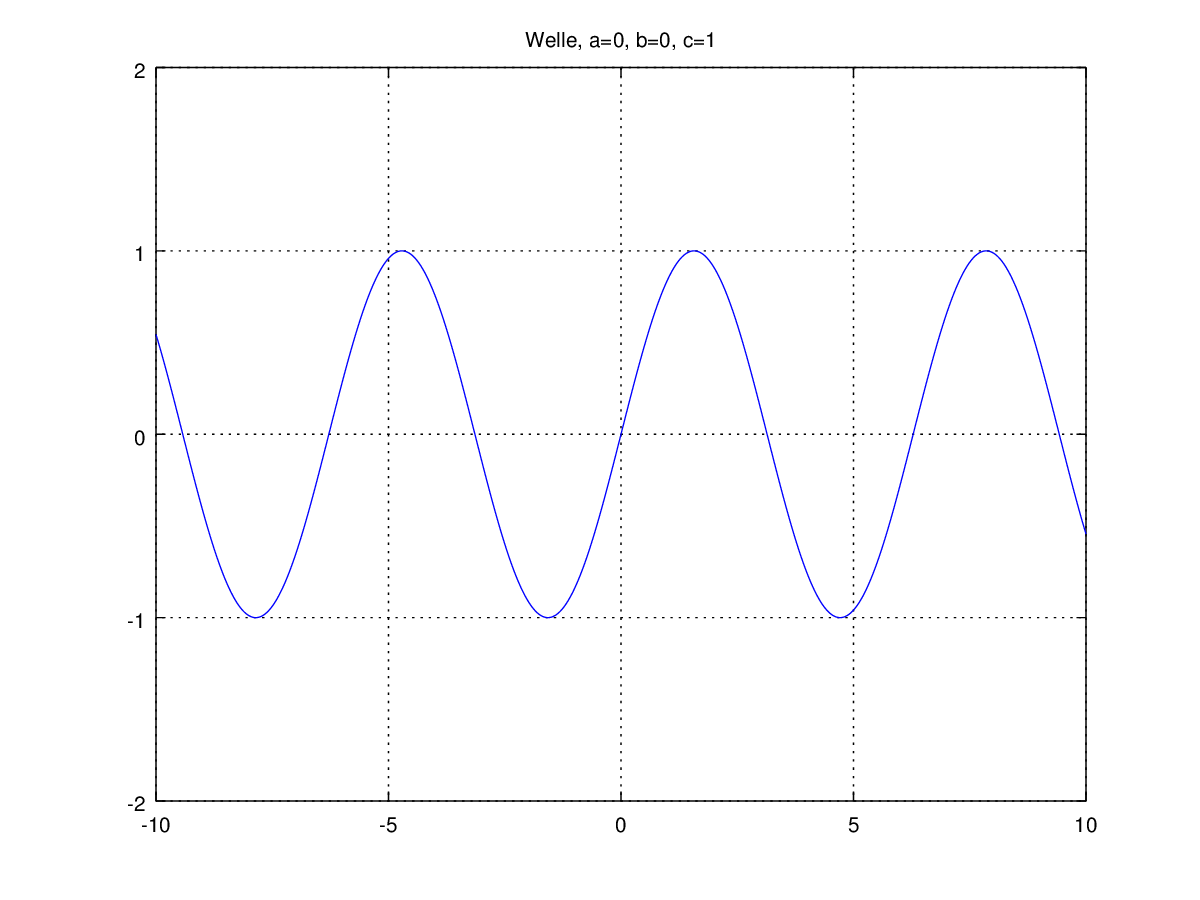
\includegraphics[width=0.5\hsize]{./wellen/images/basicfunctions/sin.png}
	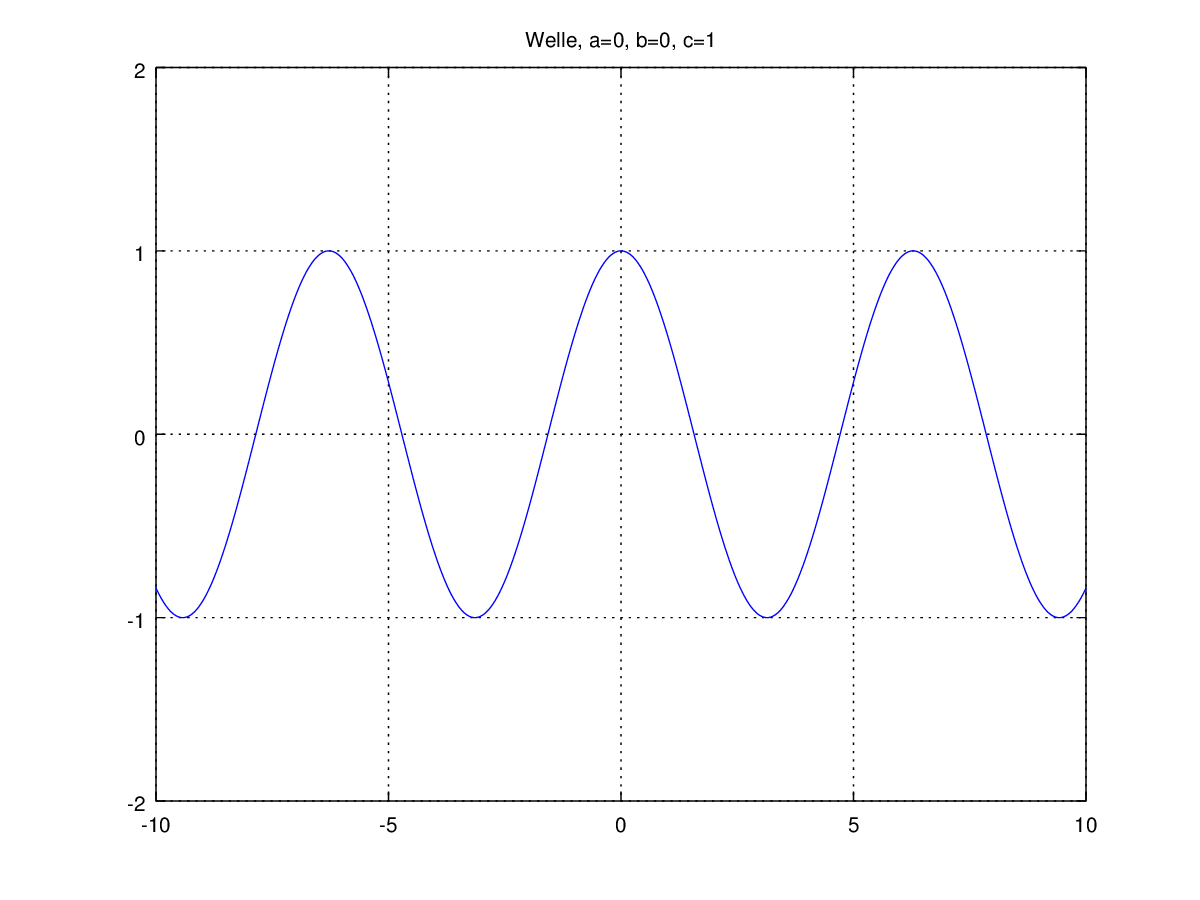
\includegraphics[width=0.5\hsize]{./wellen/images/basicfunctions/cos.png}
	\caption{$\sin$ (l.) und $\cos$ (r.)}
	\label{fig:wellen:sin-cos}
\end{figure}

\begin{figure}
	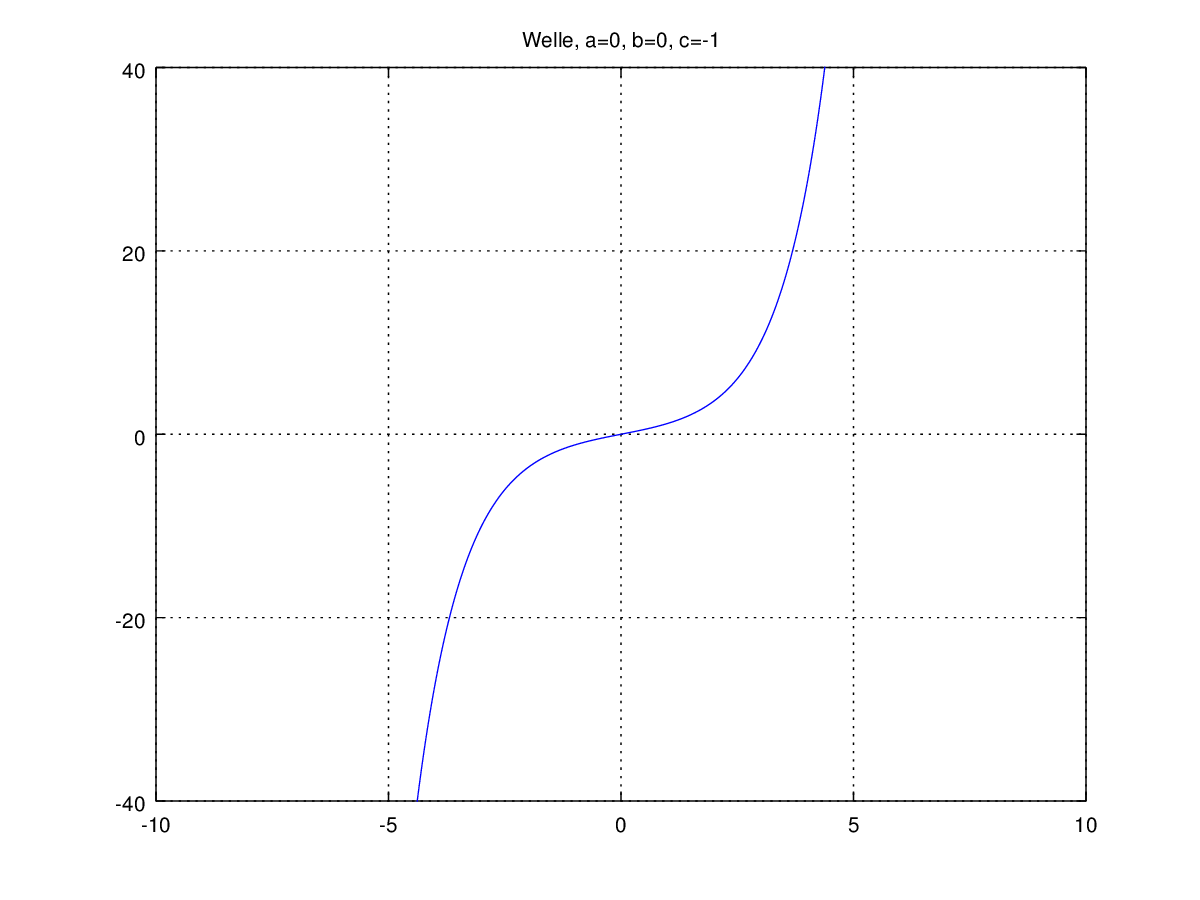
\includegraphics[scale=0.35]{./wellen/images/basicfunctions/sinh.png}
	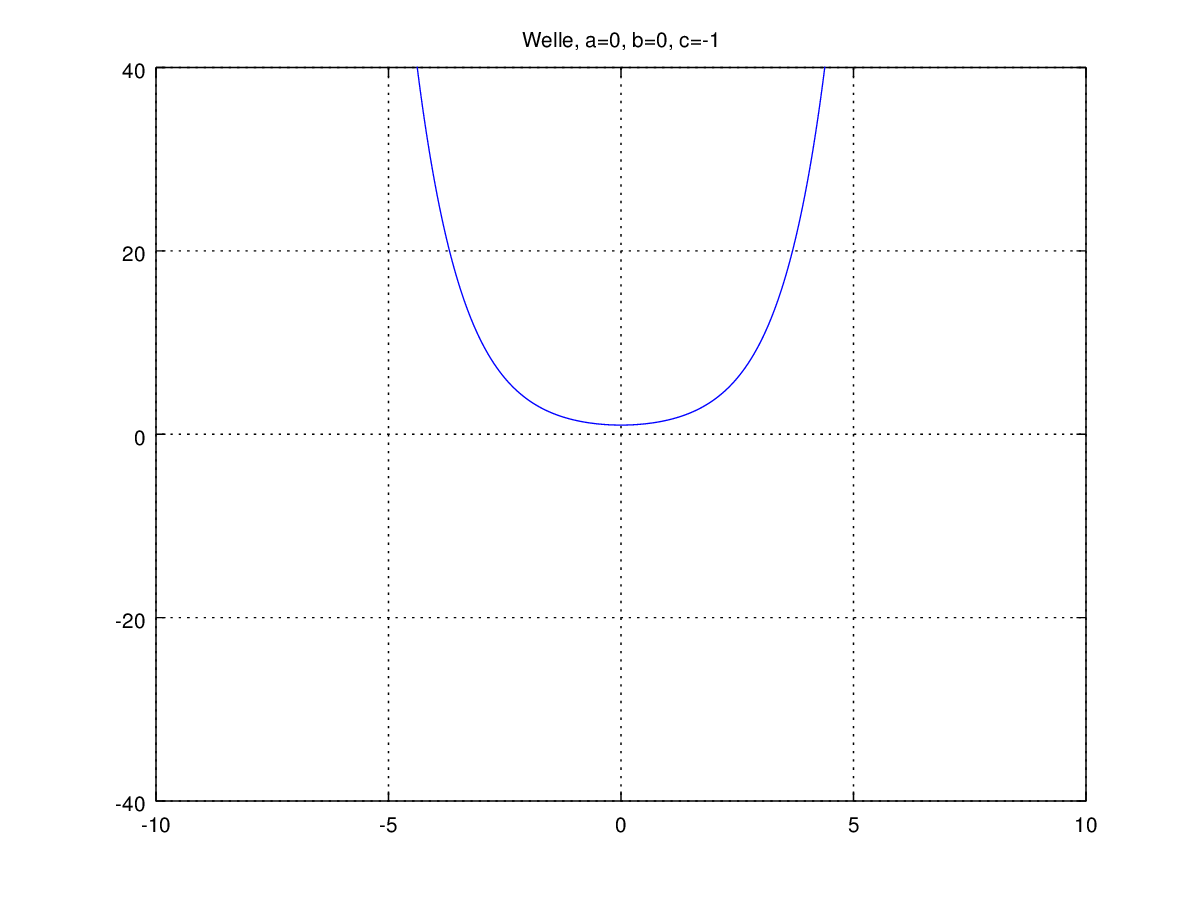
\includegraphics[scale=0.35]{./wellen/images/basicfunctions/cosh.png}
	\caption{$\sinh$ (l.) und $\cosh$ (r.)}
	\label{fig:wellen:sinh-cosh}
\end{figure}
\subsection{\texorpdfstring{$y(x) = \sum_{k = 0}^{\infty} a_{k}x^k$}{y(x) = 
summe k = 0 bis unendlich ak xk}}
\label{subsec:wellen:Potenzreihenansatz}

Als n"achstes gehen wir zur"uck auf das parabolische Kanalprofil und suchen 
L"osungen f"ur die Differentialgleichung. Dazu wird der im 
Kapitel~\ref{chapter:potenzreihen} kennengelernte Potenzreihenansatz angewandt.
Zuerst wird die Potenzreihe f"ur $y(x)$ aufgestellt und zweimal abgeleitet, da 
in der Gleichung~\eqref{eq:wellen:pxdgl} die zweite Ableitung vorkommt.
\begin{align}
	y(x)
	&=
	\sum_{k = 0}^{\infty} a_{k}x^k
	=
	a_0 + a_1x + a_2x^2 + a_3x^3 + a_4x^4 + a_5x^5 + a_6x^6 + \dotsb
	\label{eq:wellen:nullteableitung}
	\\
	y'(x)
	&=
	\sum_{k=0}^{\infty} a_{k+1}(k+1)x^k
	=
	a_1 + 2a_2x + 3a_3x^2 + 4a_4x^3 + 5a_5x^4 + 6a_6x^5+ \dotsb
	\\
	y''(x)
	&=
	\sum_{k = 0}^{\infty} a_{k+2}(k+1)(k+2)x^k
	=
	2a_2 + 3 \mathbin{\cdot} 2a_3x + 4 \mathbin{\cdot} 3a_4x^2 + 5 
	\mathbin{\cdot} 4a_5x^3 + 6 \mathbin{\cdot} 5a_6x^4 + \dotsb
	\label{eq:wellen:zweiteableitung}
\end{align}
Aus den beiden Gleichungen~\eqref{eq:wellen:nullteableitung} 
und~\eqref{eq:wellen:zweiteableitung} und dem Umstellen der Anfangsgleichung in 
die Form
\begin{equation*}
	y'' = -(ax^2+bx+c)y
\end{equation*}
kann der Koeffizientenvergleich erstellt und L"osungen f"ur die $a_k$ gefunden 
werden. Statt die Koeffizienten reihenweise aufzustellen, wird der Vergleich 
mit Hilfe der Tabelle~\ref{tab:wellen:koeffizietenvergleichtabelle} gemacht. 
Dies schafft auch bei komplizierten und langen Termen eine gute "Ubersicht und 
man erkennt auf den ersten Blick, welche $a_k$ von welchen anderen abh"angen.
\begin{table}
	\centering
	\begin{equation*}
		\begin{array}{r c r | c r | c r | c r c}
		y(x) & = &
		a_0 & + & a_1x & + & a_2x^2 & + \dotsb
		\\
		\hline&&&&&&&\\[-2ex]
		y''(x) & = &
		2\cdot1 a_2 & + & 3\cdot2 a_3x & + & 4\cdot3 a_4x^2 & + \dotsb
		\\
		& = &
		& & & + &- aa_0x^2 & + \dotsb
		\\
		& &
		& + &- ba_0x & + &- ba_1x^2 & + \dotsb
		\\
		& + &
		-ca_0 & + &- ca_1x & + &- ca_2x^2 & + \dotsb
		\\
		\hline&&&&&&&\\[-2ex]
		& &
		a_2 = -\frac{1}{2 \cdot 1}ca_0
		& & a_3 = -\frac{1}{3 \cdot 2}(ba_0+ca_1)
		& & a_4 = -\frac{1}{4 \cdot 3}(aa_0+ba_1+ca_2)
		& \dots
		\end{array}
	\end{equation*}
	\caption{Koeffizientenvergleich mittels Hilfstabelle.}
	\label{tab:wellen:koeffizietenvergleichtabelle}
\end{table}

Die Verschiebung der verschiedenen $a_k$ k"onnen folgendermassen erkl"art 
werden: Aufgrund der zweiten Ableitung werden die $a_k$ der zweiten Zeile um 
zwei Einheiten nach links geschoben. Die n"achste Verschiebung gibt es aufgrund 
des Polynomgrades. Da die Terme mit den Koeffizienten $a$ mindestens die Form 
$ax^2$ haben, verschieben sich diese um zwei Potenzen nach rechts. Die Terme 
mit den Koeffizienten $b$ haben mindestens die Form $bx^1$, daher die 
Verschiebung dieser um eine Potenz nach rechts. Einzig die Terme mit den 
Koeffizienten $c$ werden nicht verschoben, da sie mindestens als $cx^0$ 
vorhanden sind. Somit lassen sich die jeweiligen $a_k$ und ihre Abh"angigkeiten 
direkt aus den einzelnen Spalten ablesen.

Aus den in der Tabelle berechneten $a_k$ l"asst sich eine allgemeine 
Rekursionsformel
\index{Rekursionsformel}%
\begin{align*}
	a_{k+2} &= -\frac{1}{(k+2)(k+1)} (aa_{k-2}+ba_{k-1}+ca_k) \\
	\Leftrightarrow \qquad
	a_k &= -\frac{1}{k(k-1)} (aa_{k-4}+ba_{k-3}+ca_{k-2}), \qquad k \in 
	\mathbb{N} \setminus \{0, 1\}
	&&&a_{k<0} &= 0
\end{align*}
aufstellen.

\subsection{Wellendiskussion}
\label{sec:wellen:diskussionwellenform}
W"ahrend wir anschliessend mit der Rekursionsformel L"osungen unserer 
Differentialgleichung geplottet haben, entdeckten wir, dass die Welle ihre Form 
bei den jeweiligen Nullstellen des Profils $p(x)$ wechselt. Vergleichen wir die 
Wellenformen der Abbildungen \ref{fig:wellen:variablec} und 
\ref{fig:wellen:variablea} mit den Abbildungen \ref{fig:wellen:sin-cos} und 
\ref{fig:wellen:sinh-cosh}, stellt sich heraus, dass die L"osung der 
Titelgleichung eng mit der gefundenen L"osung der Gleichung 
(\ref{eq:wellen:lineareDGL}) verwandt ist. So k"onnen die L"osungen des 
Parabelprofils als verschiedene $c$ Werte der linearen Differentialgleichung 
verstanden werden, welche dann in die L"osungsgleichung 
(\ref{eq:wellen:loesunglineareDGL}) eingesetzt werden k"onnen. 
Da aber mit einem $c$, respektive mit einer L"osung des Profils nur ein Punkt 
und nicht die ganze Funktion beschrieben wird, lassen sich die Konstanten $C_1$ 
und $C_2$ aus der Gleichung (\ref{eq:wellen:loesunglineareDGL}) nicht mehr 
allgemein bestimmen. Es gibt ausserdem keine reinen trigonometrischen Formen 
mehr, sondern geht die Welle f"ur negative Profill"osungen in die 
hyperbolischen Funktionen Sinus Hyperbolicus und Cosinus Hyperbolicus und f"ur 
positive in Sinus und Cosinus über.

Die Wellenformen sind bei variablem $c$ (Abbildung \ref{fig:wellen:variablec}) 
und $a$ (Abbildung \ref{fig:wellen:variablea}) alle "ahnlich, da sich nichts 
weiteres ver"andert als der Ort der Nullstelle der Parabel. Es "andert sich die 
Wellenl"ange, vor allem wenn die Parabel weiter ge"offnet wird. Die Amplitude 
hingegen wird haupts"achlich vom $c$-Wert beeinflusst. Weiter ist erkennbar, 
dass die Profilform die Frequenz der Welle beeinflusst.

\begin{figure}
	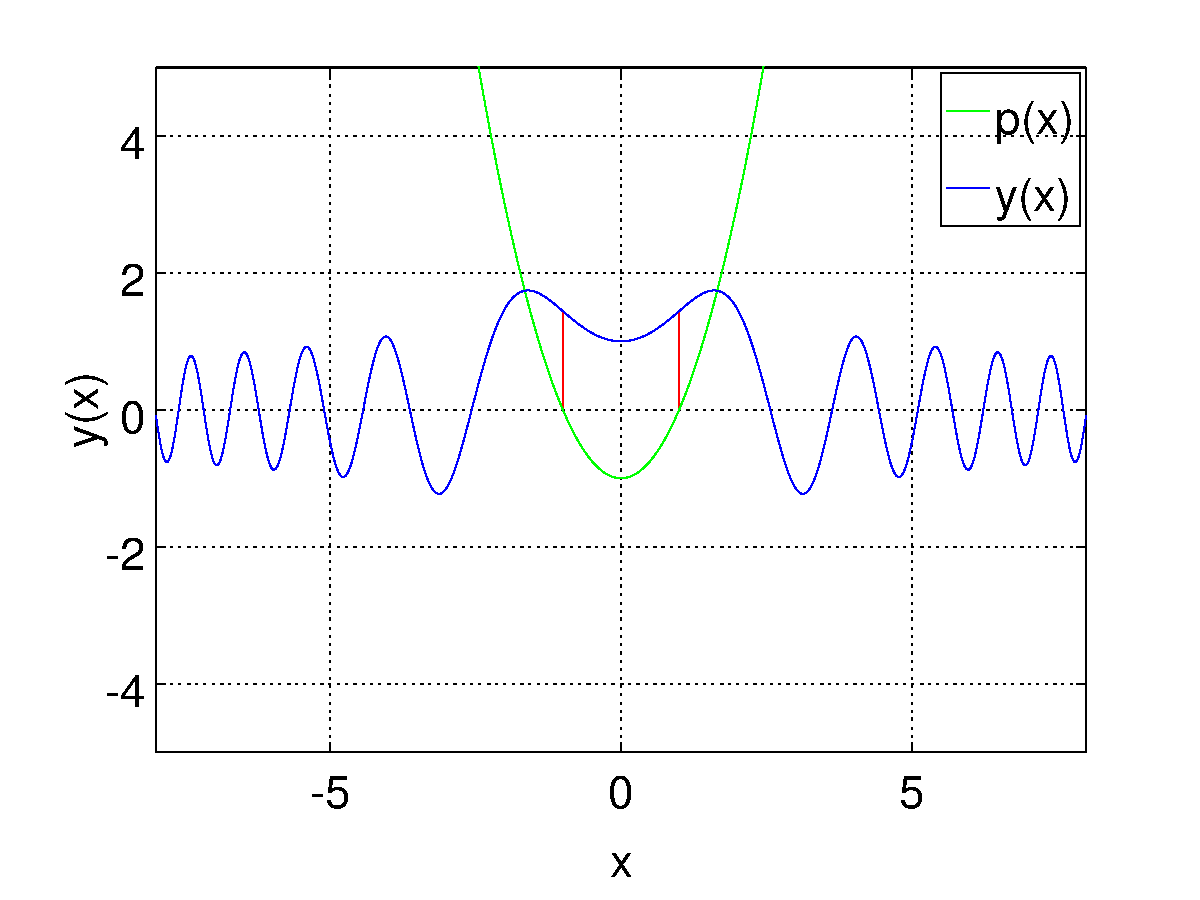
\includegraphics[width=0.51\hsize]{./wellen/images/varc/varc1.pdf}
	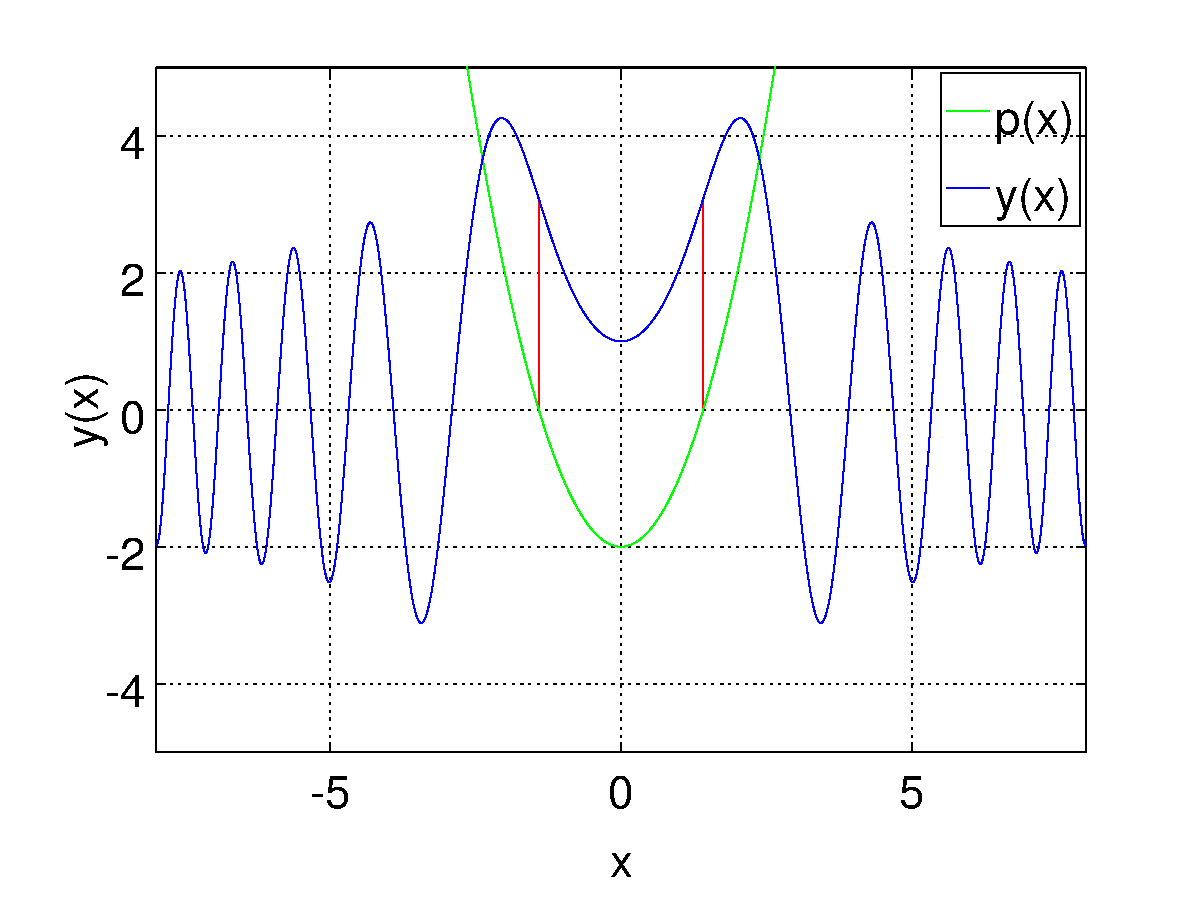
\includegraphics[width=0.51\hsize]{./wellen/images/varc/varc2.pdf}
	\caption{Wellenform mit unterschiedlichen $c$ Werten}
	\label{fig:wellen:variablec}
\end{figure}

\begin{figure}
	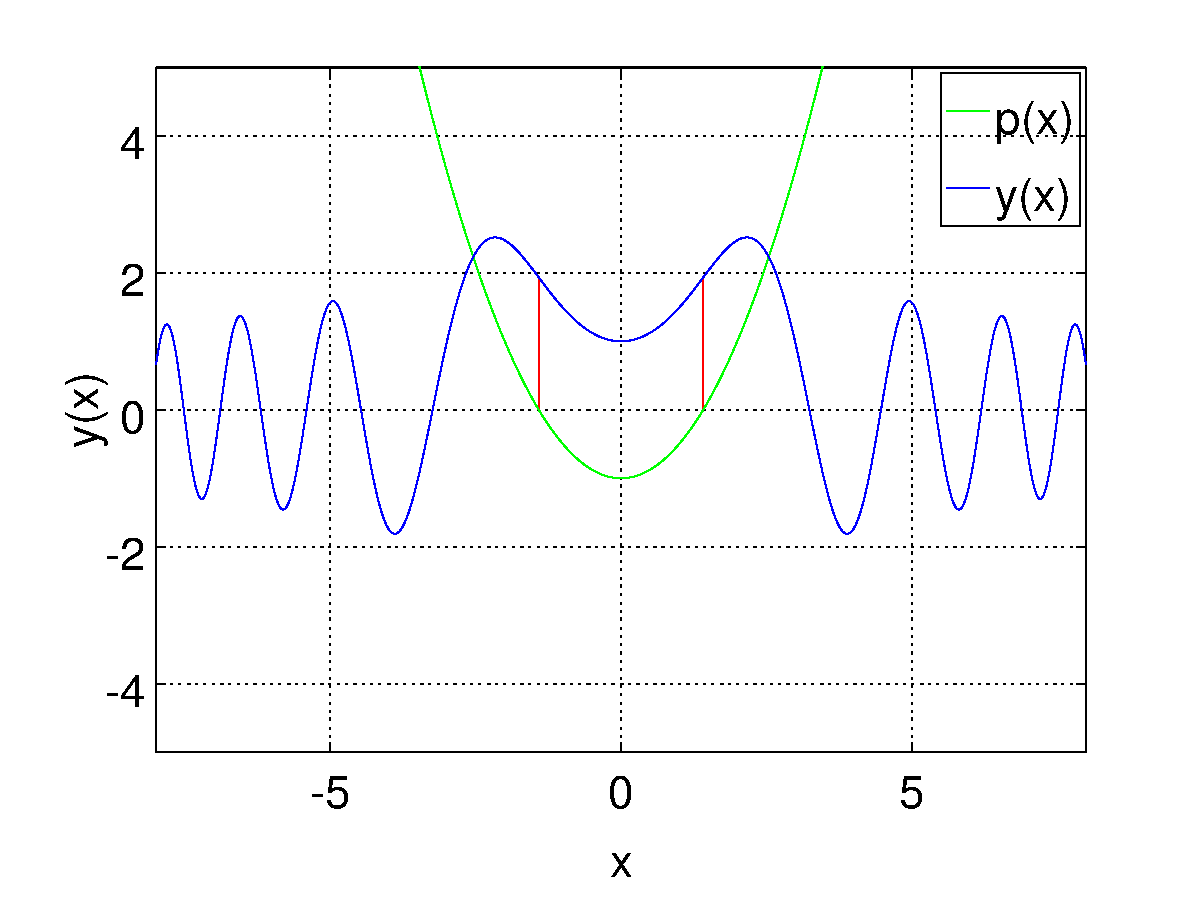
\includegraphics[width=0.51\hsize]{./wellen/images/vara/vara1.pdf}
	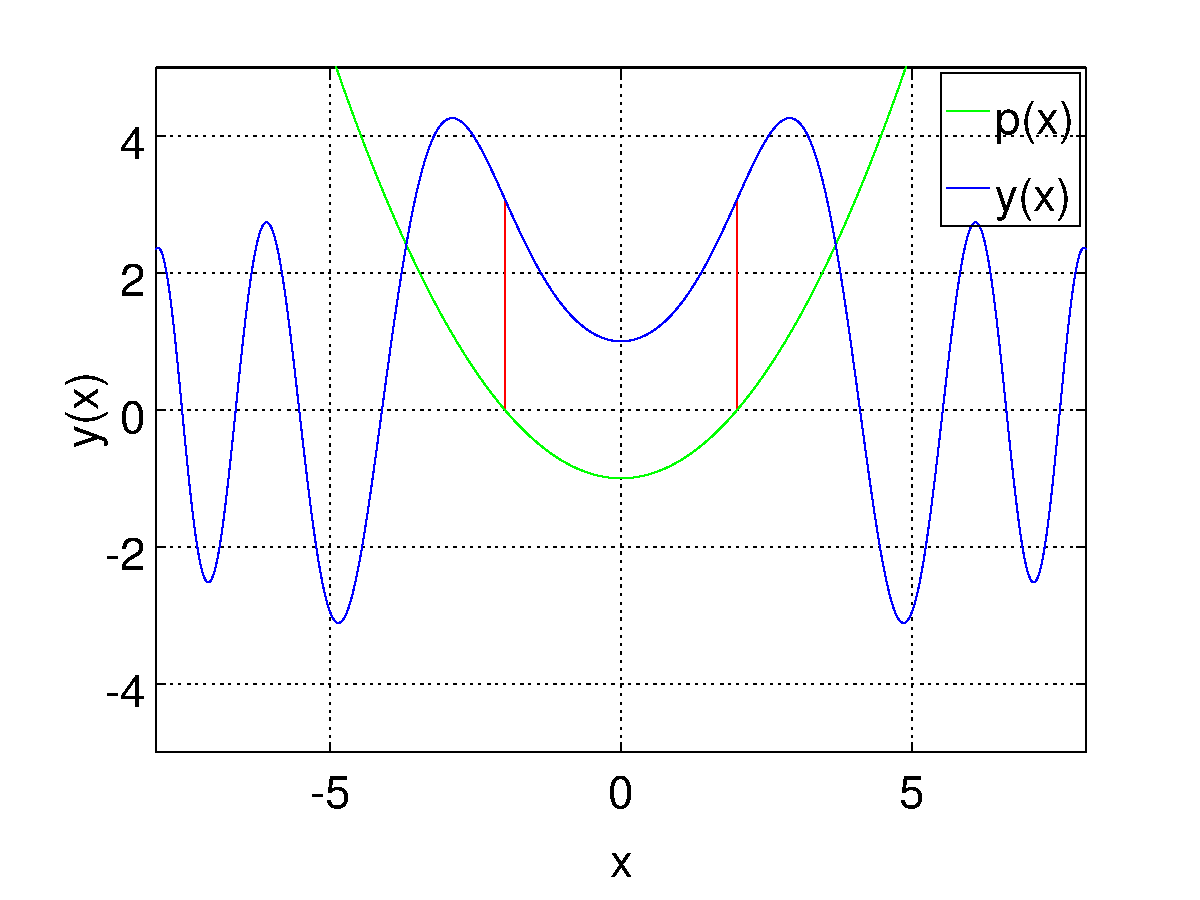
\includegraphics[width=0.51\hsize]{./wellen/images/vara/vara2.pdf}
	\caption{Wellenform bei unterschiedlichen $a$ Werten}
	\label{fig:wellen:variablea}
\end{figure}

Mit dieser Diskussion verlassen wir das parabolische Profil und betrachten 
allgemeinere Aspekte wie Stolpersteine bei der Ausf"uhrung solcher Berechnungen 
oder, die verallgemeinerte L"osung von Differentialgleichungen 
dieser Art mit einem Profil der Form
\begin{equation*}
p(x) = \sum_{i=0}^{n} \lambda_i x^i.
\end{equation*}

